% !TeX spellcheck = en_US
\chapter{Exploration}

In the setting of delayed reward, not knowing which actions would give more reward, we would want the agent to \textit{explore}. The concerns are:
\begin{itemize}
	\item How can an agent discover high-reward strategies that require a temporally extended sequence of complex behaviors that, individually, are not rewarding?
	\item How can an agent decide whether to attempt new behaviors (to discover ones with higher reward) or continue to do the best things it knows so far?
\end{itemize}
This poses a exploration and exploitation dilemma:
\begin{itemize}
	\item \textit{Exploration}: doing things you haven't done before, in the hopes of getting even higher reward
	\item \textit{Exploitation}: doing what you know will yield the highest reward
\end{itemize}

\section{Bandits Problems}
\subsection{One-Armed Bandit}
One armed bandit is the slot machine. It can be represent as a \ac{MDP} with one single action. The \ac{prob} distribution of the reward is unknown.
\begin{align}
	&\mathcal{A} = \{\text{pull arm}\}\\
	&r(\text{pull arm}) = ?
\end{align}

\begin{figure}[hbt!]
	\centering
	\includegraphics[width=.2\textwidth]{one-armed-bandit.png}
	\caption{One-armed bandit (\href{https://www.amazon.com/Armed-Bandit-Slot-Machine-Bank/dp/B001KYV9DW}{src}).}
\end{figure}

\subsection{Multi-Armed Bandit}
Multi armed bandit is a bank of multiple one-armed bandit slot machines. Different machines have different reward distribution. This problem is a 1-step stateless \ac{MDP}
\begin{align}
	&\mathcal{A} = \{\text{pull}_1, \text{pull}_2, \dots, \text{pull}_n\}\\
	&r(a_n) = ?\\
	&\text{assume } r(a_n) \sim p(r|a_n)
\end{align}

\subsection{Contextual Bandits}
the reward distribution depends on some external measurable variable.

\subsection{Bandit Variants}
\begin{itemize}
	\item Infinite Arms: there are more slot machines.
	\item Variable Arms: the reward distribution varies for each slot machine.
	\item Combinatorial Bandits: the agent has to pull more than one arm at once.
	\item Dueling Bandits: agent always pulls two arms, is never told about the reward, \dots
	\item Continuous Bandits: agent has to choose interval value, like the force to the arm.
	\item Adversarial Arms: the agent plays against an opponent. Thus if the agent uses the same strategy, the opponent will adapt, and the Q-value of that action will change over time. \Eg: chess, tic-tac-toe.
	\item Strategic Arms
	\item and more!
\end{itemize}

\subsection{Applications}
There are various applications in:
\begin{itemize}
	\item Ad serving: arms - possible ads, reward - a click
	\item Website optimization: arms: possible website options, reward - user engagement
	\item Clinical trials: arms: possible medications, reward - health outcomes
\end{itemize}

\section{Regret}
\hlb{Definition:} \textit{Regret} is the reward difference from optimal policy at time step $T$:
\begin{align*}
	&Reg(T) = T. \mathbb{E}[r(a^*)] - \sum_{t=1}^T r(a_t) && \text{regret}\\
	&\mathbb{E}[r(a^*)] && \text{expected reward of best action}\\
	&\sum_{t=1}^T r(a_t) && \text{the actual sum of reward}
\end{align*}

\hlb{Example:} Consider the following multi-armed bandit problem:\\
A professor moves to a small town for work. He will stay there for 300 days. Each day, he will eat at one of three restaurants in the town. Eating at each restaurant has a different happiness distribution. Let say, the happiness distributions of each restaurant are as follows:
\begin{itemize}
	\item Restaurant 1: $\mu=10, \sigma=5$
	\item Restaurant 2: $\mu=8, \sigma=8$
	\item Restaurant 3: $\mu=5, \sigma=25$
\end{itemize}
\textbf{Not knowing the true happiness distribution, which strategy should the professor follow to maximize the expected happiness score?}

The regrets for some exploration strategies:
\begin{itemize}
	\item Optimal reward: Knowing the true distribution, the optimal action is to always go to restaurant 1.
	\[ \mathbb{E}[r] = 300 \times 10 = 3000\]
	\item Explore only: the professor spends 100 days at each restaurant.
	\begin{align*}
		\mathbb{E}[r] &= 100 \times 10 + 100 \times 8 + 100 \times 5 = 2300\\
		\Rightarrow \rho &= 3000 - 2300 = 700 && \text{regret}
	\end{align*}
	\item Exploit only: visit each restaurant once, then stick with the one with the highest value.\\
	Assume the receive reward after 3 days are: $r_1 = 7, r_2 = 8, r_3 = 5$. After that, the expected reward would be:
	\[ \mathbb{E}[r] = 7 + 8 + 5 + (300 - 3) \times 8 = 2396 \]
	However, this is not the actual expected reward for the exploit only strategy. Thus would not be used to calculate the regret. The actual one is:
	\[\rho = 3000 - 2670 = 330\]
	\item $\epsilon$-greedy: Assume $\epsilon = 10\%$, the professor spend 10\% of the days (30 days) to explore the distribution, and the rest to exploit the current belief.
	\[\rho \approx 100\]
	\item Zero regret strategy: As time goes on $T\rightarrow \infty$, the regret will approach to 0 $\rho \rightarrow0$
\end{itemize}

\section{Optimality}
\textit{Optimality}: An exploration strategy is \textit{optimal} when we compared the regret \ac{vs} the Bayes-optimal strategy. \todo{}

\section{Tractability}
\begin{itemize}
	\item With \textit{theoretically tractable} exploration strategy, we can quantify or understand whether the given exploration strategy is optimal or sub-optimal
	\item With \textit{theoretically intractable} exploration strategy, we cannot make the above estimate exactly.
\end{itemize}

\begin{center}
	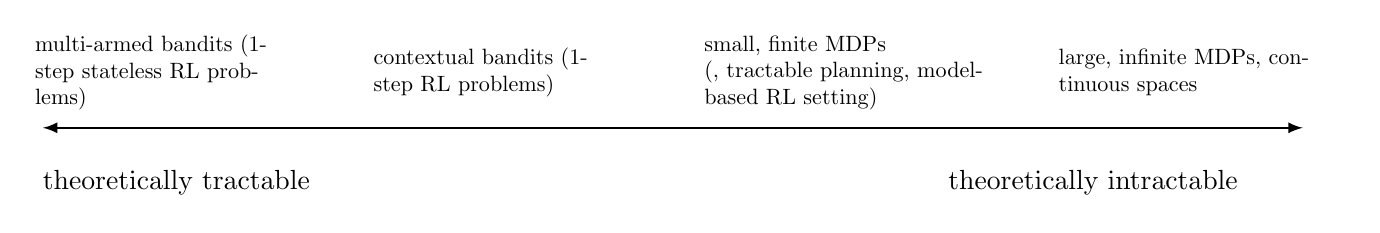
\begin{tikzpicture}
		\draw[thick,latex-latex] (-8,0) -- (8,0);
		\node[text width=5cm] at (-5.5,-.7) {theoretically tractable};
		\node[text width=5cm] at (6,-.7) {theoretically intractable};			
		\node[scale=0.8, text width=4cm] at (-6.5,.7) {multi-armed bandits (1-step stateless \ac{RL} problems)};
		\node[scale=0.8, text width=4cm] at (-2.2,.7) {contextual bandits (1-step \ac{RL} problems)};
		\node[scale=0.8, text width=4.5cm] at (2.2,.7) {small, finite \ac{MDP}s\newline (\eg, tractable planning, model-based \ac{RL} setting)};
		\node[scale=0.8, text width=4cm] at (6.5,.7) {large, infinite \ac{MDP}s, continuous spaces};
	\end{tikzpicture}
\end{center}

\section{$\epsilon$-first}

\section{$\epsilon$-greedy}

\section{UCB}
\ac{UCB} would weigh actions based on their previous rewards and how many times they have been tested.
\[ A_t = \underset{a}{\arg\max} \left[ Q_t(a) + c\sqrt{\frac{\ln t}{N_t(a)}} \right] \]
in which $Q_t(a)$ is the current belief about the reward, $N_t(a)$ is the number of times the action $a$ was chosen, $t$ is just the number of current time step. The second term measures how uncertain we currently are about the actions.

\ac{UCB}-1 use Chernoff - Hoeffding Inequality:
\[ C_j(t) = \sqrt{\frac{\log(n)}{T_j(t	)}} \]
\[ a = \underset{a}{\arg\max} \widehat{\mu}_a + \sqrt{\frac{2\ln T}{N(a)}}\]

\ac{UCB} is more difficult than $\epsilon$-greedy to extend beyond bandits to more general \ac{RL} problems (nonstationary problems, large state spaces)

\subsection{Algorithm}
\begin{enumerate}
	\item Pull each arm once
	\item Update the reward belief
	\item Choose the arm with the highest upper confidence bound.
\end{enumerate}

\section{Gradient Bandits}
\todo{}